% CS669: Pattern Recognition
% Programming Assignment II
% Gabriel Dulac-Arnold <gabe@squirrelsoup.net>
% Johannes H. Jensen <johannj@stud.ntnu.no>
\documentclass[a4paper]{article}
\usepackage{multicol}
\usepackage{graphicx}
\usepackage[top=2cm,nohead,nofoot]{geometry}

\author{Gabriel Dulac-Arnold $<$gabe@squirrelsoup.net$>$ (CS09F004) \\
Johannes H. Jensen $<$johannj@stud.ntnu.no$>$ (CS09F005) \\
\\
(Batch no. 14)}
\title{CS669 - Pattern Recognition\\
\emph{Programming Assignment III}}

\begin{document}
\setlength{\parskip}{2ex}
\setlength{\tabcolsep}{8pt}
\renewcommand\arraystretch{1.5}
\maketitle

\section{Dataset I: Linearly Separable}

These are the linearly seperable datasets that allow us to visualize the basic functioning of the various linear classifiers.
All the classifiers perform well on these datasets except for one outlying point that consistently gets misclassified for methods other than SVM.

\subsection{Classifier Accuracy}

\begin{tabular}{ | l | r | }
\hline
\textbf{Classifier} & \textbf{Accuracy} \\
\hline
Fisher Discriminant  &   99.73\% \\
\hline
Perceptron          &   99.73\% \\
\hline
SVM                 &   100\%   \\
\hline
\end{tabular}


\subsection{Confusion Matrices}

\begin{multicols}{2}
\begin{enumerate}
\item Fisher Discriminant:

\begin{tabular}{ | l | c | c | c | }
\hline
& $\omega_1$ & $\omega_2$ & $\omega_3$ \\
\hline
  $\omega_1$ & 124 & 1 & 0 \\
\hline
  $\omega_2$ & 0 & 125 & 0 \\
\hline
  $\omega_3$ & 0 & 0 & 125 \\
\hline
\end{tabular}

\item Batch Perceptron:

\begin{tabular}{ | l | c | c | c | }
\hline
& $\omega_1$ & $\omega_2$ & $\omega_3$ \\
\hline
  $\omega_1$ & 124 & 0 & 1 \\
\hline
  $\omega_2$ & 0 & 125 & 0 \\
\hline
  $\omega_3$ & 0 & 0 & 125 \\
\hline
\end{tabular}
\columnbreak

\item Support Vector Machine:

\begin{tabular}{ | l | c | c | c | }
\hline
& $\omega_1$ & $\omega_2$ & $\omega_3$ \\
\hline
  $\omega_1$ & 125 & 0 & 0 \\
\hline
  $\omega_2$ & 0 & 125 & 0 \\
\hline
  $\omega_3$ & 0 & 0 & 125 \\
\hline
\end{tabular}


\end{enumerate}
\end{multicols}


\newpage
\subsection{Decision Region Plots}

\begin{figure}[htbp!]
\center
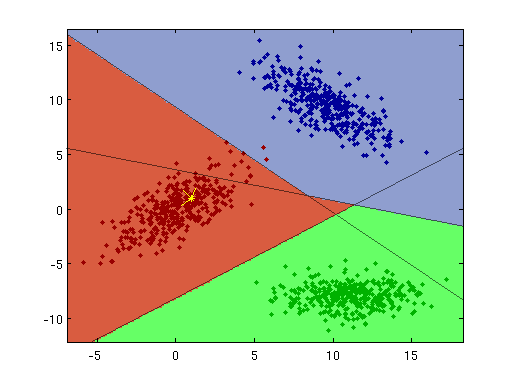
\includegraphics[clip, trim=40px 15px 30px 10px]{ls_fisher.png}
\caption{Fisher Discriminant}
\end{figure}

\begin{figure}[htbp!]
\center
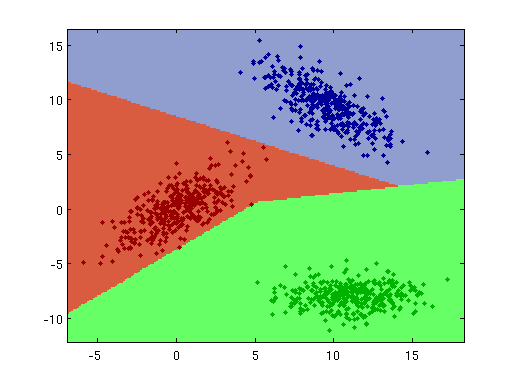
\includegraphics[clip, trim=40px 15px 30px 10px]{perceptron.png}
\caption{Perceptron}
\end{figure}

\pagebreak
\begin{figure}[htbp!]
\center
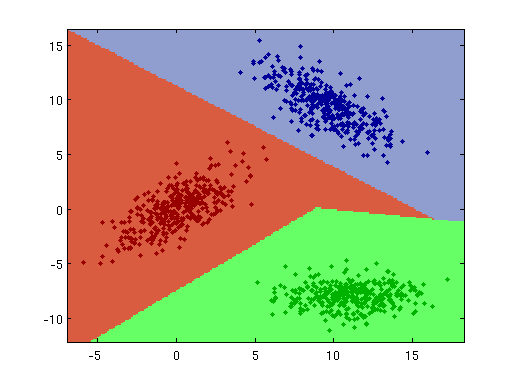
\includegraphics[clip, trim=40px 15px 30px 10px]{svm_c.png}
\caption{Support Vector Machine}
\end{figure}	

\pagebreak
\section{Dataset II: Overlapping Data}
SVM outperforms Fisher Discrimnant on the overlapping data task most likely because it is doing
a better job at maximizing the margins between the datasets.
\subsection{Classifier Accuracy}

\begin{tabular}{ | l | r | }
\hline
\textbf{Classifier} & \textbf{Accuracy} \\
\hline
Fisher Discriminant  &   89.6\% \\
\hline
SVM          &   91.2\% \\
\hline

\end{tabular}

\subsection{Confusion Matrices}

\begin{multicols}{2}
\begin{enumerate}
\item Fisher Discriminant:

\begin{tabular}{ | l | c | c | c | }
\hline
& $\omega_1$ & $\omega_2$ & $\omega_3$ \\
\hline
  $\omega_1$ & 108 & 16 & 1 \\
\hline
  $\omega_2$ & 2 & 116 & 7 \\
\hline
  $\omega_3$ & 10 & 3 & 112 \\
\hline
\end{tabular}

\item Support Vector Machine:

\begin{tabular}{ | l | c | c | c | }
\hline
& $\omega_1$ & $\omega_2$ & $\omega_3$ \\
\hline
  $\omega_1$ & 111 & 11 & 3 \\
\hline
  $\omega_2$ & 4 & 116 & 5 \\
\hline
  $\omega_3$ & 7 & 3 & 115 \\
\hline
\end{tabular}

\end{enumerate}
\end{multicols}

\subsection{Decision Region Plots}

\begin{figure}[htbp!]
\center
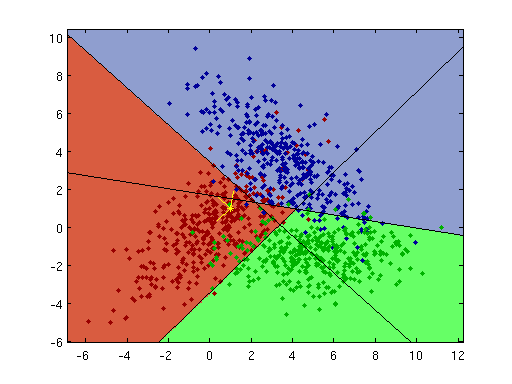
\includegraphics[clip, trim=40px 15px 30px 10px]{nls_fisher.png}
\caption{Fisher Discriminant}
\end{figure}

\begin{figure}[htbp!]
\center
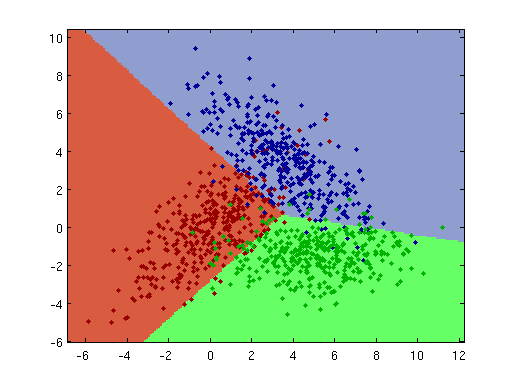
\includegraphics[clip, trim=40px 15px 30px 10px]{svm_d.png}
\caption{Support Vector Machine}
\end{figure}


\newpage


\section{Dataset III: Real World Image Feature Data}

\subsection{Classifier Accuracy}

\begin{tabular}{ | l | r | }
\hline
\textbf{Classifier} & \textbf{Accuracy} \\
\hline
Bayes Single Gaussian  &   58.67\% \\
\hline
Bayes PCA Gaussian (1 Dim.)  &   60.00\% \\
\hline
Fisher Discriminant  &   70.67\% \\
\hline
SVM          &   65.33\% \\
\hline
SVM w/ PCA & 61.33\% \\
\hline
\end{tabular}


\subsection{Confusion Matrices}

\begin{multicols}{2}
\begin{enumerate}

\item Bayes Single Gaussian:

\begin{tabular}{ | l | c | c | c | }
\hline
& $\omega_1$ & $\omega_2$ & $\omega_3$ \\
\hline
  $\omega_1$ & 20 & 1 & 4 \\
\hline
  $\omega_2$ & 10 & 7 & 8 \\
\hline
  $\omega_3$ & 5 & 3 & 17 \\
\hline
\end{tabular}
\columnbreak
\item Bayes PCA Gaussian:

\begin{tabular}{ | l | c | c | c | }
\hline
& $\omega_1$ & $\omega_2$ & $\omega_3$ \\
\hline
  $\omega_1$ & 9 & 2 & 14 \\
\hline
  $\omega_2$ & 0 & 18 & 7 \\
\hline
  $\omega_3$ & 3 & 4 & 18 \\
\hline
\end{tabular}
\columnbreak
\item Fisher Discriminant:

\begin{tabular}{ | l | c | c | c | }
\hline
& $\omega_1$ & $\omega_2$ & $\omega_3$ \\
\hline
  $\omega_1$ & 16 & 2 & 7 \\
\hline
  $\omega_2$ & 3 & 20 & 2 \\
\hline
  $\omega_3$ & 1 & 7 & 17 \\
\hline
\end{tabular}

\item Support Vector Machine

\begin{tabular}{ | l | c | c | c | }
\hline
& $\omega_1$ & $\omega_2$ & $\omega_3$ \\
\hline
  $\omega_1$ & 18 & 1 & 6 \\
\hline
  $\omega_2$ & 3 & 21 & 1 \\
\hline
  $\omega_3$ & 5 & 10 & 10 \\
\hline
\end{tabular}

\item SVM w/ PCA

\begin{tabular}{ | l | c | c | c | }
\hline
& $\omega_1$ & $\omega_2$ & $\omega_3$ \\
\hline
  $\omega_1$ & 11 & 3 & 11 \\
\hline
  $\omega_2$ & 0 & 19 & 6 \\
\hline
  $\omega_3$ & 5 & 4 & 16 \\
\hline
\end{tabular}


\end{enumerate}
\end{multicols}


\section{Conclusions}

In this assignement we see the performance of linear classifiers with gradually more complex datasets.  We don't use explicitly non-linear datasets as these would of course not work well with these techniques, but we do realize that for real-world high-dimensional applications, linear classifiers and dimensional reduction techniques work much better than Gaussian Bayes classifiers.  

We come to the conclusion that SVM and Fisher Discrimninant Analysis are the best performing classifiers for overlapping
data or high-dimensionality data, and we see that in the case of the 45 dimensional data Fisher Discriminant actually outperforms SVM, whereas the lower-dimensional problem is better handled by SVM.

\end{document}

